\section{Plugin 1: ``Hello World''}
\label{sect:plugin_1}
\subsection{Aim}
\label{ssect:plugin_1_aim}
\par %Overview and aim of this exercise
The aim of this section is to delineate the major components of QGIS python plugins and show how these components interact. To that end the reader is guider through the creation of a very basic plugin that executes very simple python code: It writes messages, including "Hello world!", in a file. This plugin is useless, but its purpose is to expose the reader to the basics of Quantum GIS plugins, by putting down the minimum amount of code. This way we avoid extensive PyQt usage.
%Code already available in the repository but the real value is in doing things yourself.
\subsection{Creating and running the plugin}
\label{ssect:creating_plugin_1}
\par %First step, create some files
The first step is to create some files. Carry out the following steps:
\begin{enumerate}
  \item Inside the \lstinline{QGIS_tutorial} directory create a directory named \lstinline{plugin_1}.
  \item Inside directory \lstinline{plugin_1} create the following files
  \begin{enumerate}
    \item \lstinline{icon.png}: Issue \lstinline{git command} to fetch a PNG file from our repository.
    \item \lstinline{__init__.py}: Use the touch utility to create an empty file.
    \item \lstinline{plugin_1.py}: Use the touch utility to create an empty file.
    \item \lstinline{metadata.txt}: Use the touch utility to create an empty file.
  \end{enumerate}
  The files listed above are mandatory.
\end{enumerate}
Next we populate the empty files, starting with \lstinline{__init__.py}. As mentioned in section \label{sect:introduction} QGIS plugins are implemented as python packages, so the \lstinline{__init__.py} file is the initialisation of the python package--class. Open the file with the editor of your choice and add the following content:
\lstinputlisting[language=Python]{../src/plugin_1/__init__.py}
\par%The python plugin code
Next lets populate the \lstinline{plugin_1.py} file. Add the following content:
\lstinputlisting[language=Python]{../src/plugin_1/plugin_1.py}
The first three functions above are mandatory. Explain functionality
\par%The plugin metadata file
The last file we need to populate is \lstinline{metadata.txt}. Add the following content:
\lstinputlisting{../src/plugin_1/metadata.txt}
\par%'install' the plugin
So far we have created code in a directory of our choosing. However, for QGIS to run any plugin in a linux machine the direcory \lstinline{plugin_1} must be placed in any of the following locations:
\begin{enumerate}
  \item \lstinline{qgis_prefix/share/qgis/python/plugins/}
  \item \lstinline{\$HOME/.qgis/python/plugins/}
\end{enumerate}
where  \lstinline{qgis_prefix} is usually \lstinline{/usr} or \lstinline{/usr/local}. Note that copying to the first directory above requires super--user priviledges and has the effect of a ``system--wide'' installation, as the plugin will be available to anyone using QGIS on that computer. Copying to the second directory will affect an installation available only to the specific user. Locate your \lstinline{qgis_prefix/share/qgis/python/plugins/} direcory. Then, if you have super--user priviledges, create link to \lstinline{plugin_1} directory from \lstinline{/usr/share/qgis/python/plugins/}. Assuming \lstinline{qgis_prefix} is \lstinline{/usr} one has to do:
\begin{lstlisting}
sudo ln -s /path/to/QGIS_tutorial/plugin_1 /usr/share/qgis/python/plugins/plugin_1
\end{lstlisting}
If the reader does not have super--user priviledges, a link from their home directory to the \lstinline{QGIS_tutorial/plugin_1} will work just as well. We avoid copying the code, instead a link was made so that whenever we modify the code we need not copy it again. Obviously this is usefull for development and training, but once a ``finished'' plugin has been developed a full copy must be placed in one of the aforementioned directories.
\par%'run' the plugin
We are now ready to load and run our plugin. Start a QGIS instance and click on ``Plugins'' on the menu bar, then select ``Manage Plugins'' as shown in figure \ref{fig:loading_QGIS_plugins}. The ``QGIS Plugin Manager'' window will appear, listing plugins ``installed'' in the system as shown in figure \ref{fig:loading_QGIS_plugins}. The tick-mark next to a plugin indicates that the plugin is ``loaded''. Clearly, we here make the distiction between installing and loading the plugin as the former being code available in an appropriate directory and the latter being an instance of the plugin class in QGIS.
\begin{figure}
 \centering
 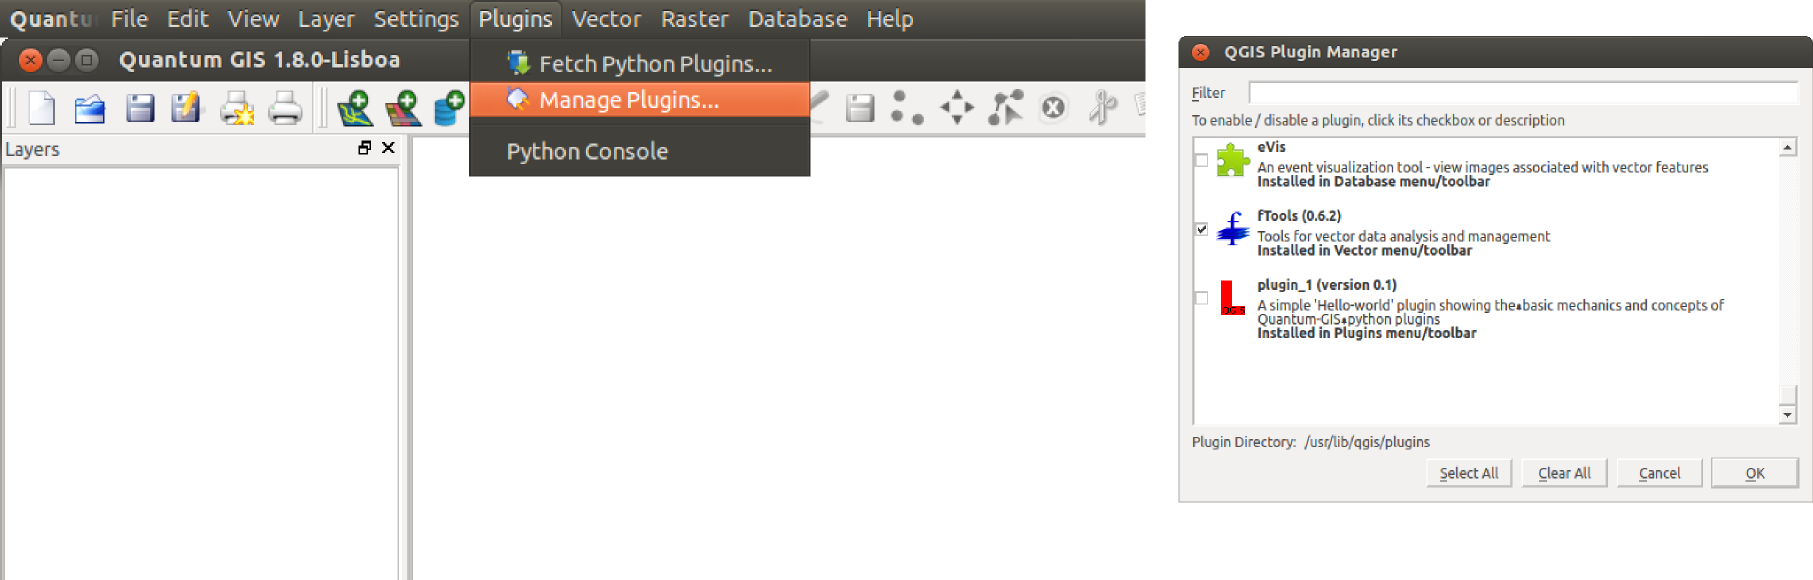
\includegraphics[width=\textwidth]{figures/loading_QGIS_plugins.png}
 \caption{Left panel; The QGIS Plugin drop--down--menu. Right panel: The ``QGIS Plugin Manager'' window.}
 \label{fig:loading_QGIS_plugins}
\end{figure}
load and run plugin steps go here.

\begin{lstlisting}
Loading plugin_1 into QGIS.
Initialising plugin_1 instance.
plugin_1 instance created, returning to QGIS.
Changing QGIS GUI to reflect plugin addition.
Hello World!
Hello World!
Resetting QGIS GUI to prior plugin-addition state. Bye World, see you soon!
\end{lstlisting}

\subsection{Understanding the basics of QGIS plugins}
\label{ssect:understanding_plugin_basics}
\par%Overview of QGIS-plugin communication.
Overview
\par%The metadata.txt file
We now turn to a closer examination of the contents of the files we created in the previous section, starting with \lstinline{metadata.txt}. 
\par%The __init__.py file
When the plugin is ``loaded'' into QGIS the module encapsulating the pluging is loaded. As such, the functions inside \lstinline{__init__.py} are called. These methods allow QGIS to obtain information on the plugin as well as create an instance of the class encapsulating the plugin. Note that the names of the functions are set and cannot be arbitrarily chosen, QGIS will attempt to call exactly these functions. The first $7$ fuctions defined in \lstinline{__init__.py} are self-explanatory. Function \lstinline{classFactory} however, deserves special attention. Its definition shows that it requires a single argument, \lstinline{interface}. This must be an instance of the \lstinline{QgisInterface} class, wich encapsulates the QGIS GUI; methods of this class allow the user to control the QGIS window. Returning to the \lstinline{classFactory} method, we see that the class \lstinline{plugin_1} from file \lstinline{plugin_1.py} is imported. The following file I/O lines will allow us to identify when this functions is executed when loading the plugin. Indeed the first line in the \lstinline{plugin_1.log} file is clearly created by method \lstinline{classFactory}. Next, an instance of the \lstinline{plugin_1} class is created--we will examine this procedure shorlty, but lets stay with \lstinline{classFactory} for now. Note that the \lstinline{plugin_1} module was imported in the first line of the \lstinline{classFactory} method. Next, another message is written to the log-file and the plugin-class instance is returned.
\par%The __init__ and initGui methods of plugin_1.py
Now lets look at file \lstinline{plugin_1.py}. The second line in \lstinline{plugin_1.log} is written from method \lstinline{__init__} in \lstinline{plugin_1} class. As mentioned above the \lstinline{classFactory} method creates an instance of the \lstinline{plugin} class, and then returns it to QGIS. Therefore, the order of the first three messages in \lstinline{plugin_1.log} is as expected. Next, QGIS calls the \lstinline{initGui} method of the plugin class. Looking at the implementation of \lstinline{initGui} we see that a message is witten to the log-file, indeed appearing in the fourth line. The following lines in \lstinline{initGui} add a button to the toolbar and a menu entry to allow for the plugin to be ``run'' when the user clicks on those entities. Setting-up this functionality requires the user to create special objects that encapsulate a click-able entity on screen: The entity has a visual repesentation as a button so it must be drawn on screen and special loops must be put in place checking if the user has clicked on the button, and then emmit a signal indicating this action. Also, other loops must continualy check for the emmition of the aforementioned signal, and take action accordingly. Fortunatelly much of this is created and handled via the PyQt library. So, after the doc-string at the top of the \lstinline{plugin_1.py} file, modules \lstinline{QtCore} and \lstinline{QtGui} are imported from package \lstinline{PyQt4}. So an ``icon'' object is first created using the \lstinline{PyQtGui.QIcon} method, and then an ``action'' is created using the \lstinline{PyQtGui.QAction} method. Note that the \lstinline{PyQtGui.QAction} method is here given a thrird argument: \lstinline{self.interface.mainWindow()}. This must be an instance of the PyQt \lstinline{QObject} class, and it is the parent object of the action. So we see that the \lstinline{QgisInterface} class also wraps PyQt object functionality; as QGIS documentation states QGIS is built using PyQt. However the reader may now be confused by the ``icon'' and ``action'' classes. What do they each do exactly? I leave this as an exercise to the reader: Examine their documentation and try to understand these objects. Some ``clues'' are given in this text. Classes \lstinline{PyQtGui.QIcon} and \lstinline{PyQtGui.QAction} do not draw anything on the QGIS main window; that is the purpose of the next two statements in the \lstinline{initGui} method of our plugin. There we invoke methods of the \lstinline{interface} object to draw a tool-bar icon and add a menu entry. The final statement in \lstinline{initGui} links the aforementioned ``action'' to a ``signal'' and a method. In general a PyQt action can emit several signals. The \lstinline{PyQtCore.QObject.connect()} method connects a signal emitted from a given action to a function. In our case the function is the method \lstinline{sayHello}.
\par%The sayHello method of plugin_1.py
The \lstinline{sayHello} method is very simple. As discussed it is invoked when the user clicks on the tool-bar icon of the plugin or on the menu-entry. It simply appends the message ``Hello World!'' to the log.  Note that the attribute identifier (the name ``sayHello'' of the function) is internal to the plugin. One could choose ``run'' or ``execute'', as long as the connection to the action is made. I chose ``sayHello'' here to highlight that point.
\par%The unload method of plugin_1.py
When the user chooses to remove the plugin from QGIS, the \lstinline{unload} method of a plugin is invoked. In the implementation of \lstinline{plugin_1.py}, messages are appended to the log and the last two lines then remove the too-bar icon as well as menu entry. Once again the particulars of the methods called are left as an exercise to the reader.

\subsection{Exercises}
\label{ssect:plugin_1_exercises}
\begin{enumerate}
\item The reader has already been encouraged to explore the documentation of particular PyQt classes. The reason these classes are not fully explained is that this is not a PyQt tutorial, the focus here is on Quantum GIS python plugins. There is already an lot of information in the preceeding paragraphs, going into PyQt particulars whould bloat the material. In addition, a key characteristic of a good programer is the ability to find and assimilate information, so this exercise will help develop this skill. On the other hand, PyQt is an integral part of QGIS plugins and it should not be glossed over. Therefore, the reader should take a look at \url{http://www.riverbankcomputing.com/software/pyqt/intro} and \url{http://pyqt.sourceforge.net/Docs/PyQt4/classes.html} to find out more on PyQt in general as well as look at the documentation of the classes \lstinline{QAction}, \lstinline{QIcon} and \lstinline{QObject}.
\item For the same reasons mentioned in the previous exercise this tutorial has not covered in detail various QGIS classes. Explore the QGIS API at \url{http://www.qgis.org/api/index.html} and look up the class \lstinline{QgisInterface}
\end{enumerate}
